\documentclass{article}
\usepackage[spanish]{babel}
\usepackage[utf8]{inputenc}
\usepackage{graphicx}
\usepackage{wrapfig}
\usepackage{amssymb, amsmath}
\setlength{\parindent}{0cm}
\title{Resumen cálculo mecánico de conductores}
\author{MakerGarage}
\date{Marzo 2021}

\begin{document}

\maketitle
\begin{center}
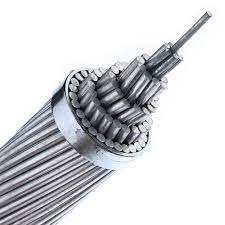
\includegraphics[trim={0 1cm 0 0},scale = 1,clip]{Conductor acero.jpg}}
\end{center}
\newpage
\tableofcontents
\newpage

\section{Pasos a seguir}
En caso de ser \textbf{categoría especial} tenemos que realizar la hipotesis de viento excepcional a la velocidad de 140km/h.
\\

Una línea se considera categoría especial en el caso de que su tensión sea igual o superior a 220 kV o que pertenezca a la red de transporte.
\subsection{Calcular los pesos en diferentes hipótesis}
Nos quedamos con el peso mas pesado para nuestra primera iteración de tensiones horizontales.

$$Peso\,del\,viento = \sqrt{P_p^2+P_v^2}$$
$P_v = 60\, ó\, 50 \cdot \left(\frac{V_v}{120} \right)^2 \cdot d \cdot 10^{-3}$
$$Peso\,del\,hielo = P_p+P_h$$
$P_h = 0'18 \,ó\, 0'36 \cdot \sqrt{d}$
\begin{equation}
    Peso\,del\,viento\, mitad = \sqrt{P_p^2+P_v^2}
\end{equation}
$P_v = \frac{60 \,ó\, 50}{2} \cdot \left(\frac{V_v}{120} \right)^2 \cdot d \cdot 10^{-3}$
\\

(1) Este se calcula en caso de tener que calcular desviación de cadena de aisladores
\subsection{Calcular la tabla de vanos añadiendo la longitud real}
$$b = \sqrt{a_i^2+h_i^2}$$
\begin{center}
\begin{tabular}{ c | c  c }

\, & Vano1 & Vano2 \\ \hline
$a_i$ & 163 & 226 \\
$h_i$ & 16 & 19 \\
$b_i$ & 163'78 & 226'80 \\
\end{tabular}
\end{center}
\subsection{Calcular el vano de regulación}
$$a_{r}=\Gamma \cdot \sqrt{\frac{\sum a_{i}{ }^{3}}{\sum \frac{b_{i}{ }^{2}}{a_{i}}}}$$
$$\Gamma=\frac{\sum \frac{b_{i}^{3}}{a_{i}^{2}}}{\sum \frac{b_{i}^{2}}{a_{i}}}$$
\newpage
\subsection{Calcular la tensión horizontal con el peso más pesado}
$$T_b = \frac{\sigma_{rotura}}{3}$$
Calculo tantas $Tm_i$ como vanos tengo.
$$T_{m i}=\frac{1}{4} \cdot\left[\left(2 \cdot T_{B}-p \cdot h\right)+\left(\sqrt{\left(p \cdot h-2 \cdot T_{B}\right)^{2}-2 \cdot b^{2} \cdot p^{2}}\right)\right]$$
Calculo los valores de $T_i$ correspondientes a cada $Tm_i$ y cogemos el valor mas pequeño.
$$T_{i}=\frac{a_{i}}{b_{i}} \cdot T_{m}$$
Definimos $t_{m 1}$ o $\tau_1$ en función de si estamos trabajando con vano único o vano de regulación respectivamente.
$$t_{m 1}=\frac{T_{m 1}}{S}$$
$$\tau_{1}=\frac{\Gamma \cdot T_{i}}{S}$$

Definimos nuestras condiciones iniciales con el peso mas pesado y ahora mediante truxa comprobaremos con el resto de hipótesis de tracción máxima admisible si efectivamente es la mas desfavorable.
\begin{center}
\begin{tabular}{| c | c | }
\hline
Condiciones iniciales & Condiciones finales \\ \hline
$\theta_1$ & $\theta_2$  \\\hline
$m_1$ & $m_2$  \\\hline
$\tau_1$ & $\tau_2$ \\\hline
\end{tabular}
\end{center}
$m = \frac{Peso\,de\,la\,hipótesis}{P_p}$\hspace{18 em}$w = \frac{P_p}{S}$
\newpage
\subsubsection{Truxa}
En función de si trabajamos con un vano único o con un vano de regulación compuesto por varios vanos, debemos calcular las condiciones iniciales.
\begin{itemize}
    \item Vano único
    
    $$t_{m 2}^{2} \cdot\left(t_{m 2}+A\right)=B$$
    $$K=\frac{a^{2} \cdot E \cdot w^{2} \cdot m_{1}^{2}}{24 \cdot t_{m 1}^{2}}-t_{m 1}$$
    $$A=\alpha \cdot E \cdot\left(\theta_{2}-\theta_{1}\right)+K$$
    $$B=\frac{a^{2} \cdot E \cdot w^{2} \cdot m_{2}^{2}}{24}$$
    \item Vano regulación
    
    $$\tau_2^{2} \cdot\left(\tau_2+A\right)=B$$
    $$K=\frac{a_{r}^{2} \cdot E \cdot w^{2} \cdot m_{1}^{2}}{24 \cdot \tau_{1}^{2}}-\tau_{1}$$
    $$A=\alpha \cdot E \cdot\left(\theta_{2}-\theta_{1}\right)+K$$
    $$B=\frac{a_{r}^{2} \cdot E \cdot w^{2} \cdot m_{2}^{2}}{24}$$
\end{itemize}
El esfuerzo en punta se puede calcular como:
$$T_{B}=T_{m}+p \cdot\left(f \cdot \frac{h}{2}\right)$$
$$T_m = \frac{b_i}{a_i} \cdot T_2$$
\\
Las flechas se pueden calcular como:
$$f=\frac{p \cdot a \cdot b}{8 \cdot T}$$
$$f=\frac{p \cdot b^{2}}{8 \cdot T_{m}}$$


\newpage
\subsection{Calcular el resto de hipótesis}
\subsubsection{EDS}
Pg 89. $m_2 = 1$ $\theta_2 = 15ºC$
$$\frac{T_B}{\sigma_{rotura}}\cdot 100 \leq 15\%$$
\begin{itemize}
    \item Calculamos $T_2$ con Truxa
    \item Calculamos tantas $Tm_i$ como vanos tengamos $T_m = \frac{b}{a}\cdot T_2$
    \item Calculamos tantas $T_{Bi}$ como vanos tengamos $T_B_i = T_m + p\cdot \left(\frac{b_i^2\cdot p}{8 \cdot Tm_i}+\frac{h_i}{2}\right)$
\end{itemize}
Nos quedamos con la $T_{Bi}$ mas grande y comprobamos que cumple la hipótesis.
\subsubsection{CHS}
Pg - No viene. $m_2 = 1$ $\theta_2 = -5ºC$
Procedimiento igual que la EDS solo que nos dan otro porcentaje.
\subsubsection{Flecha Máxima}
Pg 89-90. Debemos calcularlas para 3 hipótesis. 
\\

La flecha se calcula como $f=\frac{p \cdot a \cdot b}{8 \cdot T}$
\begin{itemize}
    \item Flecha máxima de viento
    \item Flecha máxima de hielo
    \item Flecha máxima de temperatura
\end{itemize}
\subsubsection{Flecha Mínima}
Pg 108 $m_2 = 1$. El proceso es igual que el de flecha máxima.
\subsubsection{Desviación de cadena de aisladores}
Pg 106. Debemos calcular el peso del conductor con la hipótesis de viento mitad, por tanto la sobrecarga $m_2$ tenemos que calcularla.
\end{document}
